\chapter{The \alphat Analysis}
\label{ch:5}

% **************************** Define Graphics Path **************************
\ifpdf
    \graphicspath{{Chapter5/Figs/Raster/}{Chapter5/Figs/PDF/}{Chapter5/Figs/}}
\else
    \graphicspath{{Chapter5/Figs/Vector/}{Chapter5/Figs/}}
\fi


%********************************** % First Section  *************************************
\section{Analysis Overview}  %Section - 1.1 
\label{sec:selection_analysis_overview}

Analyses searching in the jets and \met final state encounter significant 
backgrounds from SM sources of both genuine and fake \met. Genuine \met 
originates from W and Z boson production, decaying with one or more neutrinos in
the final state. In this analysis backgrounds predictions are made for these
processes using 
extrapolations into the signal region fromindependent, process-specific control
samples, as described at length in chapter~\ref{ch:6}.
Fake \met predominantly is found due to mismeasurements of QCD 
multijet (MJ) events, which are the dominant process in the hadronic environment and 
phase space considered in this analysis due to very large cross sections. 
Small inconsistencies in the handling of such large backgrounds or rare detector
effects can therefore 
have a significant impact on an analysis. This background is reduced to an 
entirely negligible level using the dimensionless kinematic variable, \alphat
(later described in section~\ref{sec:alphat}).

% OLD
% Analyses searching in the jets and \met final state encounter significant 
% backgrounds from SM sources of both genuine \met, originating from the leptonic 
% decays of W bosons, 
% and fake \met, originating from jet mis-measurement. The \alphat 
% analysis makes predictions for the former using a data-driven transfer factor 
% technique to extrapolate yields from statistically independent control samples 
% into the signal region. However the latter, sources of fake \met from QCD multijet events,
% are reduced to a negligible level using the kinematic 
% variable \alphat.

In this analysis events are binned in exclusive categories of \HT, 
and the multiplicity of jets and b-tagged jets,  
\nj and \nb, as summarised in table~\ref{tab:ht-bins}. Such binning allows for
targeted interpretations across the vast array of
possible simplified model final states, while reducing background yields to a 
minimum.

\begin{table}[ht!]
  \caption{\HT binning used for each \nj and \nb category.\label{tab:ht-bins}}
  \centering
  % \scriptsize % too big to fit on page
  \tiny
  \begin{tabular}{ lrrrrrrrrrrr }
    \hline
    \hline
    (\nj,\nb)       & \multicolumn{11}{c}{\HT bins (\gev)}                                                                                \\
    \hline
    (2-3,0)           & 200--275 & 275--325 & 325--375 & 375--475 & 475--575 & 575--675 & 675--775 & 775--875 & 875--975 & 975--1075 & $>$1075  \\
    (2-3,1)           & 200--275 & 275--325 & 325--375 & 375--475 & 475--575 & 575--675 & 675--775 & 775--875 & 875--975 & 975--1075 & $>$1075  \\
    (2-3,2)           & 200--275 & 275--325 & 325--375 & 375--475 & 475--575 & 575--675 & 675--775 & 775--875 & $>$875   & \multicolumn{2}{c}{} \\
%    (2-3,3)          & 200--275 & 275--325 & 325--375 & 375--475 & 475--575 & 575--675 & 675--775 & 775--875 & $>$875   & \multicolumn{2}{c}{} \\
    ($\geq$4,0)       & 200--275 & 275--325 & 325--375 & 375--475 & 475--575 & 575--675 & 675--775 & 775--875 & 875--975 & 975--1075 & $>$1075  \\
    ($\geq$4,1)       & 200--275 & 275--325 & 325--375 & 375--475 & 475--575 & 575--675 & 675--775 & 775--875 & 875--975 & 975--1075 & $>$1075  \\
    ($\geq$4,2)       & 200--275 & 275--325 & 325--375 & 375--475 & 475--575 & 575--675 & 675--775 & 775--875 & $>$875   & \multicolumn{2}{c}{} \\
    ($\geq$4,3)       & 200--275 & 275--325 & 325--375 & 375--475 & 475--575 & 575--675 & 675--775 & 775--875 & $>$875   & \multicolumn{2}{c}{} \\
    ($\geq$4,$\geq$4) & 200--275 & 275--325 & 325--375 & $>$375   & \multicolumn{7}{c}{}                                                        \\
    \hline
    \hline
  \end{tabular}
\end{table}

The main analysis signal region is described in the remainder of this chapter.


\subsection{The \alphat kinematic variable}
\label{sec:alphat}

QCD multijet (MJ) events dominate the SM background in any search with multiple jets 
in the final state. Jet energy mis-measurements in a 
purely QCD MJ event can lead to non-negligible amounts of \mht, therefore 
passing the signal selection. Attempting
to accurately measure this contribution is
made very difficult given the hadronic environment of the LHC, and the lack of 
precise measurements and calculations of the large multijet cross sections. As an 
alternative approach, the goal of this analysis is to reduce QCD down to an
entirely negligible level. This is 
achieved with the dimensionless kinematic variable, \alphat. The di-jet variable
$\alpha$ was first proposed by Randall et al. in 2008 \cite{Randall:2008rw},
and later translated into the transverse plane for use with LHC analyses
\cite{CMS:2008vya, CMS-PAS-SUS-09-001}.
\alphat is defined for di-jets as:

\begin{equation}
\alphat = \frac{ \sqrt{E_T^{j_2}/E_T^{j_1}} }{ \sqrt{2(1-cos(\Delta \phi))} }
\label{eq:alphat_di-jet}
\end{equation}

where $E_T^{j_1}$ and $E_T^{j_2}$ are the reconstructed transverse energies of 
the first and second jets respectively, and $\Delta \phi$ is the seperation 
between the two jets in the $\phi$ plane.

A perfectly measured di-jet event containing back to back jets in $\phi$ of equal energy will
have an \alphat value of 0.5, whereas 
events with \met originating from jet energy mismeasurements will have values of $\alphat<0.5$.
Events containing sources of genuine \met, whether from SM or BSM sources, can have values
of $\alphat > 0.5$. REWORD?

% \begin{equation}
% \alphat = \frac{E_T^{j_2}}{M_T} = \frac{\sqrt{}}
% \label{eq:alphat_di-jet}
% \end{equation}

% where $E_T^{j_2}$ is the transverse energy of the less energetic jet and $M_T$ 
% is the transverse mass of the di-jet system, defined as:

% \begin{equation}
% M_T = \sqrt{\bigg(\sum^2_{i=1}{E_T^{j_i}}\bigg)^2 - \bigg(\sum^2_{i=1}{p_x^{j_i}}\bigg)^2 - \bigg(\sum^2_{i=1}{p_y^{j_i}}\bigg)^2}
% \label{eq:mt}
% \end{equation}

% where $E_T^{j_i}$, $p_x^{j_i}$ and $p_y^{j_i}$ are the transverse energy and 
% transverse momentum in the $x$ and $y$ planes, for the jet $j_i$.

The \alphat variable can be generalised to an n-jet case by considering the event as a 
pseudo-di-jet system, constructing each pseudo-jet such that the difference in \HT
between each pseudo-jet system, \deltaHT, is minimised. \alphat then takes the 
form:

\begin{equation}
\alphat = \frac{1}{2} \times \frac{\HT-\deltaHT}{\sqrt{\HT^2 - \mht^2}} = 
\frac{1}{2} \times \frac{1-\frac{\deltaHT}{\HT}}{\sqrt{1 - \frac{\mht}{\HT}^2}}
\label{eq:alphat_njet}
\end{equation}

\emph{show plots of correlations between \mht and \deltaHT for QCD, 
signal, SM real MET etc.}


%********************************** % First Section  *************************************
\section{Hadronic Signal Region}
\label{sec:selection_hadronic}
% Introduce that QCD is a dominant background due to jet mis-measurement.

This section outlines the relevant background sources of this analysis, and
describes the basic hadronic pre-selection made for the signal 
region, as well as the relevant trigger requirements and data and 
simulation samples used.

\subsection{Standard Model Backgrounds}

\subsubsection{Genuine \met}
The dominant EWK source of genuine missing energy comes from a Z-boson 
production where the Z decays
via neutrinos, \zinv, with associated jet production. This source of background
is considered irreducible.

Events containing leptonic decays of W bosons, \wlnu, originating either
from direct W production, or via the decay of a top quark from \ttbar 
production, are sources of genuine 
missing energy. The presence of a weakly interacting neutrino which evades
detection leads to an energy imbalance. Such events are vetoed in the signal
region due to the presence of a 
lepton, however if the lepton is missed for whatever reason, leptonic W decays 
can pass the signal selection, forming a significant SM background.

% While lepton and photon vetoes employed in the signal region suppress 
% significant amounts of background from events with neutrinos, such events can 
% still persist if, for example, the lepton is not identified.
% Such processes are predominantly from \ttbar or W-boson production, where the 
% W decays via \wlnu. If the lepton is `lost' and evades our 
% lepton vetoes, significant missing energy can be produced not only from missing 
% the lepton, but from the presence of the neutrino. When such processes are accompanied 
% by associated jet production they are then able to pass our signal region selection.

Leptons can be `lost' for a variety different reasons, but ultimately for failing
the lepton ID criteria. There are numerous potential causes, the 
most prevalent being soft-leptons below ID threshold or non-isolated leptons 
which pass the ID quality cuts but fail the isolation requirement.

Events containing a Single Isolated Track (SIT) are vetoed from the signal 
region. This tracker based veto is particularly useful for vetoing additional events 
that contain leptons which have failed our lepton ID requirements entirely, and 
are therefore not considered by the leptonic vetoes. Additionally, the veto also
removes background contributions from single-pronged hadronical decays of $\tau$
leptons.

While originally designed to target hadronically decaying tau leptons, 
this requirement reduces the remaining lost-lepton backgrounds also.

Following the reduction of such processes using the lepton, photon and SIT vetoes,
any remaining contributions from SM EWK backgrounds are estimated using a 
fully data-driven transfer factor technique, described in detail in
Section~\ref{sec:background_overview}. A breakdown of the EWK background 
composition is shown in Figure~\ref{fig:background_decomp}, split into the main 
categories of \zinv, \wj, \ttbar and other residual backgrounds.

\begin{figure}[hb!]
\centering
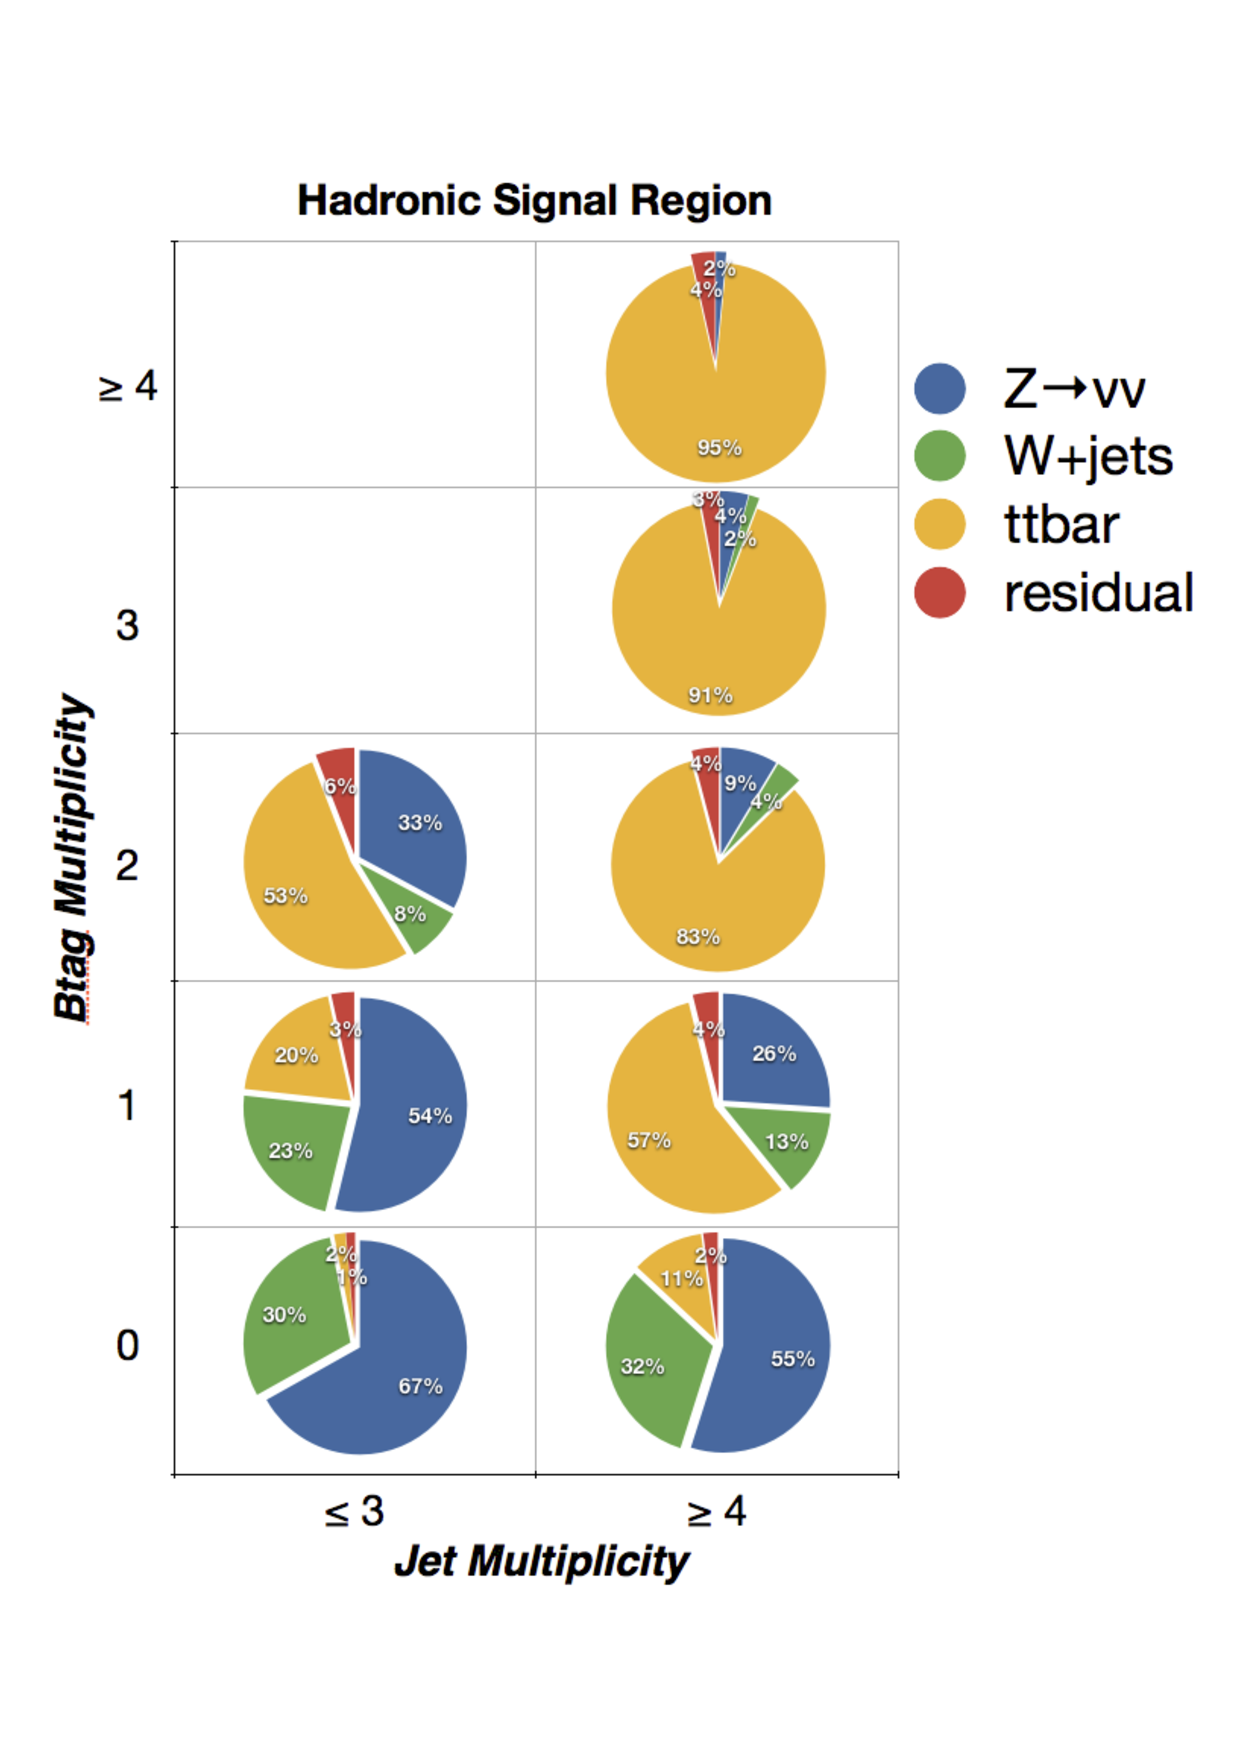
\includegraphics[width=0.7\textwidth]{Figs/ra1_had_bg_comp.pdf}
\label{fig:background_decomp}
\caption{DO}
\end{figure}

\subsubsection{Fake \met}

As mentioned previously, the dominant source of background for analyses 
searching for a multijet final state is from QCD. A fully-measured QCD event 
would consist of multiple jets balancing each other in all planes, however in 
order to enter the signal region, an event must contain missing energy, 
\mht (equivalent to \met in all-hadronic events).

The most common way for a balanced multijet (MJ) event to gain \mht is when one 
or more of the jets are mis-measured, such that their vectorial sum then leads to non-zero
\mht. This can due to detector issues, or due to stochastic fluctuations within
the inherant jet-resolution of the 
detector. The former is protected against using a filter to remove events 
affected by non-functioning or damaged regions of the ECAL system, where 
events are vetoed if they contain significant energy deposits within a given 
distance from a known problematic region. The latter is dealt with using a
cut on the \alphat variable where 
events with fake missing energy signatures give values $<0.5$.

QCD MJ events can also appear to contain non-zero missing energy 
due to the threshold requirements of jets. If an event contains 
one or more jets below the analysis threshold, then the 
event is measured as imbalanced and containing \mht. Events such as these are largely 
removed with the \alphat requirement, however in addition a requirement is made on the
ratio \mhtmet.

Finally, it is also possible for rare instrumentation effects to lead to jet 
energy
mismeasurements. To protect against this, a suite of MET filters are defined by 
the JetMET \emph{POG}, and are applied to all selections.


\subsection{Signal Triggers}

\emph{Add emphasis on parked trigger, as it opens up phase space to compressed susy models}

Events are collected at the HLT using a dedicated suite of
signal triggers. For an event to pass the trigger
requirements, it must exceed both a \HT and an \alphat threshold. Trigger rate 
can be maintained by varying the
threshold requirement on each of these independent `legs', as shown in Table~
\ref{tab:sig_trigs}. Each \HT bin in the analysis is seeded by a single trigger,
with a 25 \gev offset in online and offline \HT, with the exception of the
200 \gev bin.

% \begin{table}[h]
% \begin{tabular}{l|l}
% HT bin (\gev) & HLT Trigger            \\ \hline
% 200-275       & HLT\_HT200\_AlphaT0p57 \\
% 275-325       & HLT\_HT200\_AlphaT0p57 \\
% 325-375       & HLT\_HT300\_AlphaT0p53 \\
% 375-475       & HLT\_HT350\_AlphaT0p52 \\
% 475-575       & HLT\_HT400\_AlphaT0p51 \\
% 575-675       & HLT\_HT400\_AlphaT0p51 \\
% 675-775       & HLT\_HT400\_AlphaT0p51 \\
% 775-875       & HLT\_HT400\_AlphaT0p51 \\
% 875-975       & HLT\_HT400\_AlphaT0p51 \\
% 975-1075      & HLT\_HT400\_AlphaT0p51 \\
% 1075-$\inf$   & HLT\_HT400\_AlphaT0p51 \\
% \end{tabular}
% \label{tab:sig_trigs}
% \end{table}

\begin{table}[!ht]
  \caption{Signal triggers, the L1 seed triggers and their efficiencies measured
  for per \HT and \nj category.}
  \label{tab:sig_trigs}
  \centering
  \scriptsize
  \begin{tabular}{ cccccc }
    \hline
    \hline
    Offline \HT       & Offline \alphat & L1 seed (\verb!L1_?!)         & Trigger (\verb!HLT_?!)  & \multicolumn{2}{c}{Efficiency (\%)}          \\ [0.5ex]
    region (\gev)         & threshold       & (highest thresholds)          &                         & $2 \leq \nj \leq 3$ & $\nj \geq 4$       \\ [0.5ex]
    \hline
    $200 < \HT < 275$ & 0.65            & \verb!DoubleJetC64!           & \verb!HT200_AlphaT0p57! & $81.8^{+0.4}_{-0.4}$  & $78.9^{+0.3}_{-0.4}$ \\
    $275 < \HT < 325$ & 0.60            & \verb!DoubleJetC64!           & \verb!HT200_AlphaT0p57! & $95.2^{+0.3}_{-0.4}$  & $90.0^{+1.2}_{-1.3}$ \\
    $325 < \HT < 375$ & 0.55            & \verb!DoubleJetC64 OR HTT175! & \verb!HT300_AlphaT0p53! & $97.9^{+0.3}_{-0.3}$  & $95.6^{+0.9}_{-1.0}$ \\
    $375 < \HT < 475$ & 0.55            & \verb!DoubleJetC64 OR HTT175! & \verb!HT350_AlphaT0p52! & $99.2^{+0.2}_{-0.2}$  & $98.7^{+0.5}_{-0.7}$ \\
    $\HT > 475$       & 0.55            & \verb!DoubleJetC64 OR HTT175! & \verb!HT400_AlphaT0p51! & $99.8^{+0.1}_{-0.3}$  & $99.6^{+0.3}_{-0.7}$ \\
    \hline
    \hline
  \end{tabular}
\end{table}

Trigger efficiencies are measured against an unbiased single muon reference trigger,
\\\verb!HLT_IsoMu24_eta2p1!, using a muon tag and probe method \emph{Henning: "
hmmmm"} where a
single muon is selected and then subsequently ignored from the analysis when 
calculating event level variables such as \HT, \mht and \alphat. Efficiencies 
are measured for each \HT bin and for each \nj category, as summarised in 
table~\ref{tab:sig_trigs}. Example trigger turn on curves are shown for the 3 
lowest \HT bins in figures~\ref{fig:eff_alphat_le3j} and \ref{fig:eff_alphat_ge4j}.
Across the higher \HT 
bins the triggers are fully efficient, with some inefficiencies seen only in the
lower \HT bins. These inefficiencies are understood as being due to the L1 seed
trigger used for this region, which had high thresholds in order to maintain 
low rates in the high PU environment throughout \runone. Lower 
efficiencies are also observed in the \njhigh category attributed to the presence of 
softer jets, as an increased number of jets must equate to the same total \HT 
requirement of the bin.

\begin{figure}[!ht]
  \centering
    
    \begin{subfigure}[b]{0.48\textwidth}
      
\includegraphics[width=\textwidth,page=11]{figures/trigger/HT200_275_73_73_36_AlphaT_le3j_RunAtFNAL}
      \caption{Differential, $200 < \HT < 275 $ \gev}
    \end{subfigure}
    \begin{subfigure}[b]{0.48\textwidth}
      
\includegraphics[width=\textwidth,page=18]{figures/trigger/HT200_275_73_73_36_AlphaT_le3j_RunAtFNAL}
      \caption{Cumulative, $200 < \HT < 275 $ \gev}
    \end{subfigure} \\
    \begin{subfigure}[b]{0.48\textwidth}
      
\includegraphics[width=\textwidth,page=11]{figures/trigger/HT275_325_73_73_36_AlphaT_le3j_RunAtFNAL}
      \caption{Differential, $275 < \HT < 325 $ \gev}
    \end{subfigure}
    \begin{subfigure}[b]{0.48\textwidth}
      
\includegraphics[width=\textwidth,page=18]{figures/trigger/HT275_325_73_73_36_AlphaT_le3j_RunAtFNAL}
      \caption{Cumulative, $275 < \HT < 325 $ \gev}
    \end{subfigure} \\
    \begin{subfigure}[b]{0.48\textwidth}
      
\includegraphics[width=\textwidth,page=11]{figures/trigger/HT325_375_86_86_43_AlphaT_le3j_RunAtFNAL}
      \caption{Differential, $325 < \HT < 375 $ \gev}
    \end{subfigure}
    \begin{subfigure}[b]{0.48\textwidth}
      
\includegraphics[width=\textwidth,page=18]{figures/trigger/HT325_375_86_86_43_AlphaT_le3j_RunAtFNAL}
      \caption{Cumulative, $325 < \HT < 375 $ \gev}
    \end{subfigure} \\
  
    \caption{\label{fig:eff_alphat_le3j}
      Differential (left) and Cumulative (right) efficiency turn-on curves for 
      the signal triggers, for the three lowest \HT bins and \njlow.}
\end{figure}

\begin{figure}[!ht]
  \centering
    
    \begin{subfigure}[b]{0.48\textwidth}
      
\includegraphics[width=\textwidth,page=11]{figures/trigger/HT200_275_73_73_36_AlphaT_ge4j_RunAtFNAL}
      \caption{Differential, $200 < \HT < 275 $ \gev}
    \end{subfigure}
    \begin{subfigure}[b]{0.48\textwidth}
      
\includegraphics[width=\textwidth,page=18]{figures/trigger/HT200_275_73_73_36_AlphaT_ge4j_RunAtFNAL}
      \caption{Cumulative, $200 < \HT < 275 $ \gev}
    \end{subfigure} \\
    \begin{subfigure}[b]{0.48\textwidth}
      
\includegraphics[width=\textwidth,page=11]{figures/trigger/HT275_325_73_73_36_AlphaT_ge4j_RunAtFNAL}
      \caption{Differential, $275 < \HT < 325 $ \gev}
    \end{subfigure}
    \begin{subfigure}[b]{0.48\textwidth}
      
\includegraphics[width=\textwidth,page=18]{figures/trigger/HT275_325_73_73_36_AlphaT_ge4j_RunAtFNAL}
      \caption{Cumulative, $275 < \HT < 325 $ \gev}
    \end{subfigure} \\
    \begin{subfigure}[b]{0.48\textwidth}
      
\includegraphics[width=\textwidth,page=11]{figures/trigger/HT325_375_86_86_43_AlphaT_ge4j_RunAtFNAL}
      \caption{Differential, $325 < \HT < 375 $ \gev}
    \end{subfigure}
    \begin{subfigure}[b]{0.48\textwidth}
      
\includegraphics[width=\textwidth,page=18]{figures/trigger/HT325_375_86_86_43_AlphaT_ge4j_RunAtFNAL}
      \caption{Cumulative, $325 < \HT < 375 $ \gev}
    \end{subfigure} \\
  
    \caption{\label{fig:eff_alphat_ge4j}
      Differential (left) and Cumulative (right) efficiency turn-on curves for 
      the signal triggers, for the three lowest \HT bins and \njhigh.}
\end{figure}

\emph{explain the difference between the cumu and diff turn on curves}

All triggers were present throughout \runone, however the 
\\\verb!HLT_HT200_AlphaT0p57! trigger was used as part of the `Parked' stream of 
data which was reconstructed at a later date, following the active data-taking 
period. During data taking triggers may have `prescale' factors applied to them 
such that only every $n$ triggered events are actually recorded, however all of
the signal triggers remained unprescaled for the entirety of the 8 \tev
data-taking.


\subsection{Selection Criteria}
\label{sec:selec_crit}

Event selection for the hadronic signal region are chosen with an aim to 
maintain sensitivity to hadronically decaying sparticle production, while 
rejecting as many QCD-type processes as possible. To do so, requirements are 
made on:

\begin{description}
\item[Jets]
Events are required to contain at least two jets are required and have at least
$\HT > 200$ \gev, to ensure the presence of significant hadronic activity. As 
mentioned previously, events are categorised by \HT, with jet \Pt
requirements on the two leading and the remaining additional jets seperately.
The jet \Pt thresholds vary as a function of the \HT bin of the event, as shown in
Table~\ref{tab:jet_pt_thresholds}.

\begin{table}[ht!]
  \caption{Jet \Et thresholds per \HT bin.\label{tab:jet_pt_thresholds}}
  \centering
  \footnotesize
  \begin{tabular}{ lcccc }
    \hline
    \hline
    \HT bin    & 200--275 & 275--325 & 325--375 & $>$375 \\
    \hline
    Lead jet       & 73.3     & 73.3     & 86.7     & 100.0  \\
    Second jet     & 73.3     & 73.3     & 86.7     & 100.0  \\
    All other jets & 36.7     & 36.7     & 43.3     & 50.0   \\
    \hline
    \hline
  \end{tabular}
\end{table}

\item[Leptons]
Any events containing leptons are vetoed to ensure purely hadronic events
are considered, thereby suppressing events with genuine \met from leptonic decays to
neutrinos such as \wlnu.

\item[Photons]
Events containing photons are vetoed, for similar reasons as the leptonic 
vetoes, in order to maintain a purely hadronic environment.

\item[Event]
The topology of the event is required to pass a threshold of $\alphat > 0.55$, 
which itself varies as a function of the \HT category being considered, always 
chosen such that QCD MJ events contribute a negligible amount to the overall 
background. While no absolute \met requirement is made, the cut on 
\alphat imposes an implied threshold, which maintains the analysis'
sensitivity to very low regions of \met. \emph{give an example of the actual met
threshold for a given HT bin.}

\end{description}



It is possible for events to acquire significant amounts of \mht without having any
real \met present when multiple jets are below the analysis threshold. To protect against 
this scenario, events are required to have a low ratio of the two variables, specifically
\mhtmet < 1.25.

It is possible for events to acquire significant amounts of \mht without having any
real \met present when multiple jets are below the analysis threshold. To protect against 
this scenario, events are required to have a low ratio of the two variables, specifically
\mhtmet < 1.25.

Events can also acquire fake \mht if they overlap with areas of the calorimeter 
system which are damaged or known to be faulty, where jets can be mis-measured or 
lost as a result. To protect against this, for a given jet $j$, the angular separation
between the event \mht, calculated excluding jet $j$, and the jet itself is used, defined
as:

\begin{equation}
\dphistar_j = \Delta \phi\big(\overrightarrow{\Pt}_j,-\sum_{i\neq j}{\overrightarrow{\Pt}_i}\big)
\label{eq:biasdphi}
\end{equation}

\emph{Why is this better than $\Delta \phi(\met, jet)$?}

A small value of $\dphistar_j$ indicates that the momentum vector of $j$
is aligned with the \mht vector, implying the jet is mis-measured. Events are 
vetoed if a jet with \dphistar<0.5 is within $\Delta R < 0.3$ of a known
`dead' region of the ECAL.

Events are required to have \dphistar > 0.3, in order to clean any remaining 
events containing sources of genuine \met overlapping with a jet.
\emph{is it right to explain this is for genuine met sources as well??}

For bins of $\HT>375$ \gev the leading two jets in the event are required to 
have $\Pt>100$ \gev, with all additional jets having half the requirement of
$\Pt>50$ \gev. In order to maintain a similar kinematic phase space throughout
the many \HT bins, these jet \Pt requirements are scaled for the lower \HT bins 
as shown in Table~\ref{tab:jet_pt_thresholds}.


Example distributions of \alphat, \HT, \mht and jet \Pt  are shown in
figure~\ref{fig:datamc_had_inc}, comparing data against MC.

\begin{figure}[!ht]
  \centering
    \begin{subfigure}[b]{0.48\textwidth}
      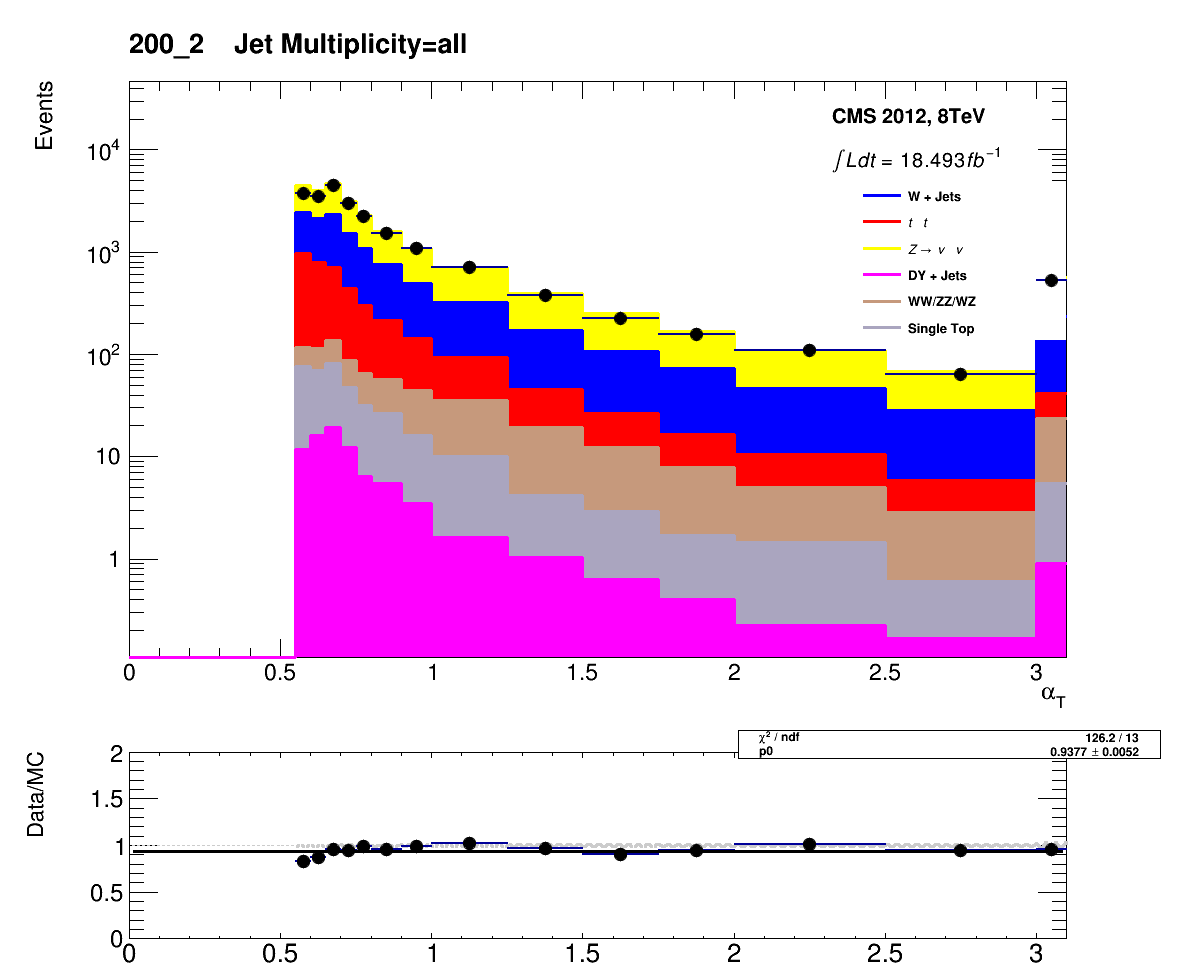
\includegraphics[width=\textwidth]{Figs/datamc/had/Stacked_AlphaT_all_200_upwards}
      \caption{\alphat}
    \end{subfigure}
    \begin{subfigure}[b]{0.48\textwidth}
      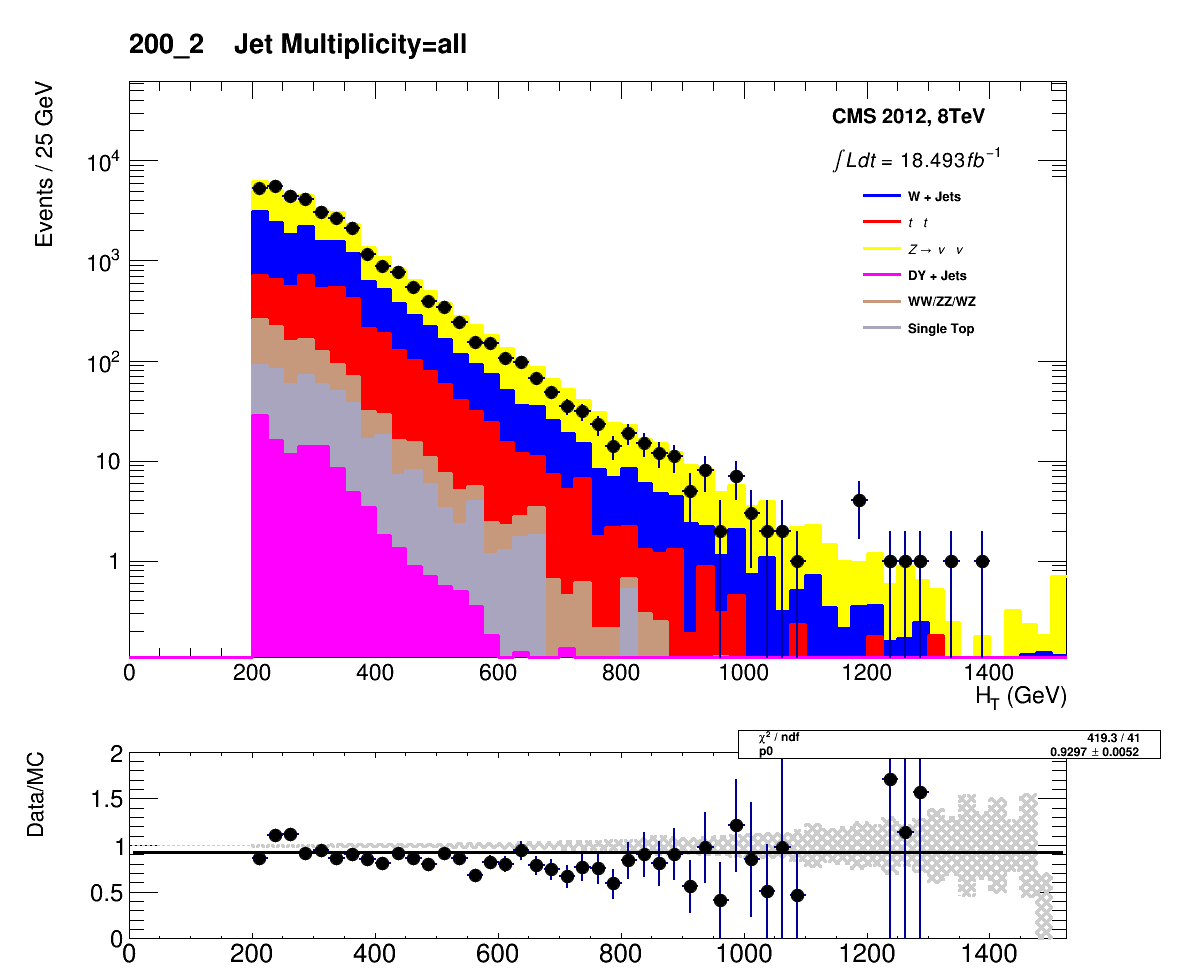
\includegraphics[width=\textwidth]{Figs/datamc/had/Stacked_HT_all_200_upwards}
      \caption{\HT}
    \end{subfigure} \\
    \begin{subfigure}[b]{0.48\textwidth}
      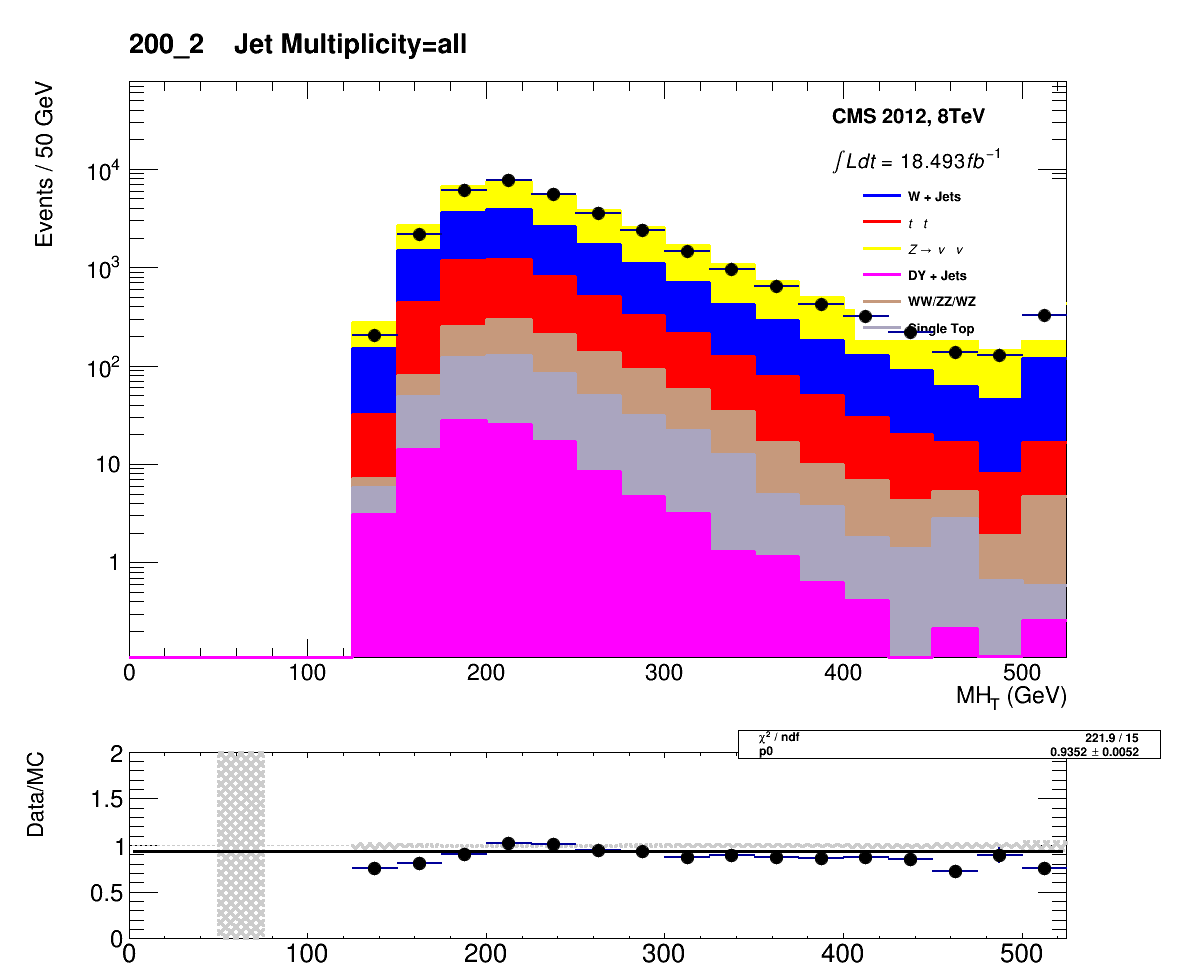
\includegraphics[width=\textwidth]{Figs/datamc/had/Stacked_MHT_all_200_upwards}
      \caption{\mht}
    \end{subfigure}
    \begin{subfigure}[b]{0.48\textwidth}
      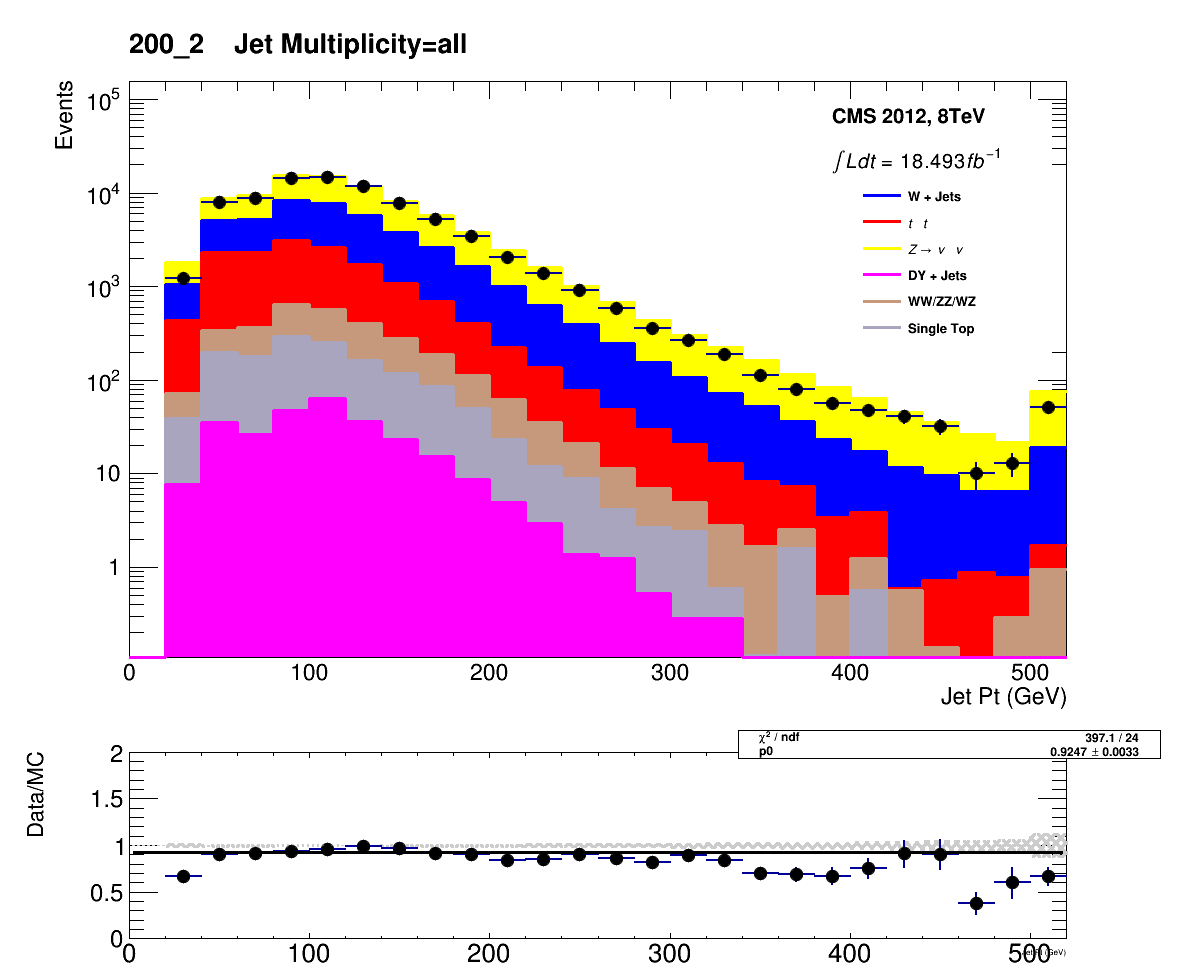
\includegraphics[width=\textwidth]{Figs/datamc/had/Stacked_CommonJetPt_all_200_upwards}
      \caption{Jet \Pt}
    \end{subfigure} \\
    \caption{\label{fig:datamc_had_inc}
    Comparison of data with MC for the full hadronic signal selection. Plots 
    are for $\HT>200$ \gev, $\nj\geq2, \nb\geq0$.
    }
\end{figure}

\emph{Cutflow with event yields after each cut}

\emph{SHOW TABLE WITH THE BACKGROUND BREAKDOWN - PUT INTO GRAPHICAL FORM?}

\subsection{Formula method}

tie in with the split into nb and nj categories - necessary as stats will reduce, so we use
this `trick' to reduce errors

